\documentclass{beamer}
%\documentclass[handout]{beamer}

\pdfcompresslevel9

\usepackage{graphicx}
\usepackage{epic}
\usepackage{epsfig}
\usepackage{eepicemu}
\usepackage{color}
\usepackage{alltt}
\usepackage{cancel}
\usepackage{hhline}
\usepackage{amssymb}
\usepackage{verbatim}
\usepackage{boxedminipage}
\usepackage{listings}
\usepackage{helvet}
\usepackage{pgf}
\usepackage{tikz}
\usepackage{xspace}
\usepackage{dsfont}
\usepackage[noend]{algorithmic}
\usepackage{mathrsfs}
\usepackage{pifont}

\hypersetup{%
	pdftitle={\inserttitle},%
	pdfauthor={\insertauthor},%
	pdfsubject={},%
	pdfkeywords={}%
}

\DeclareGraphicsExtensions{.pdftex,.png,.pdf,.jpg}
\DeclareGraphicsRule{.pdftex}{pdf}{*}{}

\begin{lrbox}{2233}
\begin{picture}(0,0)
\put(300,-20){
\includegraphics[width=2cm]{cbmc-logo-medium}}
\end{picture}
\end{lrbox}

\institute[]{
\includegraphics{cbmc-logo-medium}}

\usetheme{boxes}
\usefonttheme[stillsansseriftext,stillsansserifsmall]{serif}
\setbeamerfont{frametitle}{size=\large,series=\bfseries,shape=\sf}
\addfootbox{structure}{\,\sf{\bf \insertshorttitle} --
\href{http://www.cprover.org/}{http://www.cprover.org/}\hfill\insertframenumber\,}
\addheadbox{structure}{\usebox{2233}}

\renewcommand{\implies}{\Rightarrow}

\begingroup\makeatletter\ifx\SetFigFont\undefined%
\gdef\SetFigFont#1#2#3#4#5{%
  \reset@font\fontsize{#1}{#2pt}%
  \fontfamily{#3}\fontseries{#4}\fontshape{#5}%
  \selectfont}%
\fi\endgroup%

% COLORS

% butter (yellowish)
\definecolor{tabutter}{rgb}{0.98824, 0.91373, 0.30980}		% #fce94f
\definecolor{ta2butter}{rgb}{0.92941, 0.83137, 0}		% #edd400
\definecolor{ta3butter}{rgb}{0.76863, 0.62745, 0}		% #c4a000

% orange
\definecolor{taorange}{rgb}{0.98824, 0.68627, 0.24314}		% #fcaf3e
\definecolor{ta2orange}{rgb}{0.96078, 0.47451, 0}		% #f57900
\definecolor{ta3orange}{rgb}{0.80784, 0.36078, 0}		% #ce5c00

% chocolate (brownish)
\definecolor{tachocolate}{rgb}{0.91373, 0.72549, 0.43137}	% #e9b96e
\definecolor{ta2chocolate}{rgb}{0.75686, 0.49020, 0.066667}	% #c17d11
\definecolor{ta3chocolate}{rgb}{0.56078, 0.34902, 0.0078431}	% #8f5902

% chameleon (greenish)
\definecolor{tachameleon}{rgb}{0.54118, 0.88627, 0.20392}	% #8ae234
\definecolor{ta2chameleon}{rgb}{0.45098, 0.82353, 0.086275}	% #73d216
\definecolor{ta3chameleon}{rgb}{0.30588, 0.60392, 0.023529}	% #4e9a06

% sky blue
\definecolor{taskyblue}{rgb}{0.44706, 0.56078, 0.81176}		% #728fcf
\definecolor{ta2skyblue}{rgb}{0.20392, 0.39608, 0.64314}	% #3465a4
\definecolor{ta3skyblue}{rgb}{0.12549, 0.29020, 0.52941}	% #204a87

% plum (violettish)
\definecolor{taplum}{rgb}{0.67843, 0.49804, 0.65882}		% #ad7fa8
\definecolor{ta2plum}{rgb}{0.45882, 0.31373, 0.48235}		% #75507b
\definecolor{ta3plum}{rgb}{0.36078, 0.20784, 0.4}		% #5c3566

% scarlet red
\definecolor{tascarletred}{rgb}{0.93725, 0.16078, 0.16078}	% #ef2929
\definecolor{ta2scarletred}{rgb}{0.8, 0, 0}			% #cc0000
\definecolor{ta3scarletred}{rgb}{0.64314, 0, 0}			% #a40000

% aluminium
\definecolor{taaluminium}{rgb}{0.93333, 0.93333, 0.92549}	% #eeeeec
\definecolor{ta2aluminium}{rgb}{0.82745, 0.84314, 0.81176}	% #d3d7cf
\definecolor{ta3aluminium}{rgb}{0.72941, 0.74118, 0.71373}	% #babdb6

% gray
\definecolor{tagray}{rgb}{0.53333, 0.54118, 0.52157}		% #888a85
\definecolor{ta2gray}{rgb}{0.33333, 0.34118, 0.32549}		% #555753
\definecolor{ta3gray}{rgb}{0.18039, 0.20392, 0.21176}		% #2e3436

% gray
\definecolor{tagray}{rgb}{0.53333, 0.54118, 0.52157}		% #888a85

\usecolortheme[named=ta3skyblue]{structure}

\setbeamercolor{block body}{fg=black,bg=ta3skyblue!10}
\setbeamercolor{block title}{fg=black,bg=ta3skyblue!30}
\mode<handout>{\setbeamercolor{block body}{fg=black,bg=white!90!black}}
\mode<handout>{\setbeamercolor{block title}{fg=black,bg=white!70!black}}

\newcommand{\RETURN}{\STATE \textbf{return}~}
%\renewcommand{\ENDIF}{}

\newcommand{\power}[1]{\mathscr P({#1})}

\newcommand{\mycheck}{{\color{ta3chameleon}\ding{52}}}
\newcommand{\myfail}{{\color{ta3scarletred}\ding{56}}}


\title{CBMC: Bounded Model Checking for ANSI-C}

\date{Version 1.0, 2010}

% LTL
\def\TEMPOP#1{\mathrm{\bf #1}}
\def\X{\TEMPOP{X}}
\def\F{\TEMPOP{F}}
\def\E{\TEMPOP{E}}
\def\A{\TEMPOP{A}}
\def\G{\TEMPOP{G}}
\def\U{\mathrel{\TEMPOP{U}}}
\def\R{\mathrel{\TEMPOP{R}}}

\begin{document}

% ------------------------------------------------------------------------
% ------------------------------------------------------------------------
% ------------------------------------------------------------------------

\frame[plain]{\titlepage}

% ------------------------------------------------------------------------
% ------------------------------------------------------------------------
% ------------------------------------------------------------------------

\begin{frame}
\frametitle{Outline}
\setcounter{tocdepth}{1}
\tableofcontents
\setcounter{tocdepth}{2}
\end{frame}

% ------------------------------------------------------------------------
% ------------------------------------------------------------------------
% ------------------------------------------------------------------------

\section{Preliminaries}

\begin{frame}
\frametitle{Preliminaries}

\begin{itemize}

\item We aim at the analysis of programs given in a
commodity programming language such as C, C++, or Java
\vfill

\item As the first step, we transform the program
into a \emph{control flow graph} (CFG)

\end{itemize}

\vfill

\begin{center}
\scalebox{.75}{\input{frontend.xfigtex}}
\end{center}

\end{frame}

% ------------------------------------------------------------------------
% ------------------------------------------------------------------------
% ------------------------------------------------------------------------

\lstset{language=C,basicstyle=\rmfamily\tiny,escapechar=\$,columns=flexible}

\begin{frame}[fragile]
\frametitle{Example: SHS}

\begin{columns}
\begin{column}{.7\textwidth}
\begin{lstlisting}[language=C,
basicstyle=\rmfamily\tiny,escapechar=\$,columns=flexible]
if ( (0 <= t) && (t <= 79) )
  switch ( t / 20 )
  {
  case 0:
     TEMP2 = ( (B AND C) OR (~B AND D) );
     TEMP3 = ( K_1 );
     break;

  case 1:
     TEMP2 = ( (B XOR C XOR D) );
     TEMP3 = ( K_2 );
     break;

  case 2:
     TEMP2 = ( (B AND C) OR (B AND D) OR (C AND D) );
     TEMP3 = ( K_3 );
     break;

  case 3:  
     TEMP2 = ( B XOR C XOR D );
     TEMP3 = ( K_4 );
     break;

  default: 
     ${\colorbox{tabutter}{\rmfamily assert(0);}}$
  }
\end{lstlisting}
\end{column}
\begin{column}{.3\textwidth}
\pause
\includegraphics{sha-example-0}
\end{column}
\end{columns}

\end{frame}

% ------------------------------------------------------------------------
% ------------------------------------------------------------------------
% ------------------------------------------------------------------------

\begin{frame}
\frametitle{Bounded Program Analysis}

Goal: check properties of the form $\A\G p$,\\
say assertions.
\vfill

Idea: {\color{ta3skyblue}follow paths through the CFG} to an assertion,\\
and build a formula that corresponds to the path

\end{frame}

% ------------------------------------------------------------------------
% ------------------------------------------------------------------------
% ------------------------------------------------------------------------

\begin{frame}
\frametitle{Example}

\begin{columns}
\begin{column}{.3\textwidth}
\only<1| handout:0>{\includegraphics{sha-example-0}}%
\only<2->{\includegraphics{sha-example-1}}
\end{column}
\begin{column}{.1\textwidth}
\pause\pause

\includegraphics[width=\textwidth]{arrow}
\end{column}
\begin{column}{.6\textwidth}
$\begin{array}{ll}
      & 0 \le t \le 79 \\
\land & t/20\not=0 \\
\land & t/20=1 \\
\land & \mathit{TEMP2}=B \oplus C \oplus D \\
\land & \mathit{TEMP3}=K\_2
\end{array}$
\end{column}
\end{columns}

\end{frame}

% ------------------------------------------------------------------------
% ------------------------------------------------------------------------
% ------------------------------------------------------------------------

\begin{frame}
\frametitle{Example}

We pass

\[ \begin{array}{ll}
      & 0 \le t \le 79 \\
\land & t/20\not=0 \\
\land & t/20=1 \\
\land & \mathit{TEMP2}=B \oplus C \oplus D \\
\land & \mathit{TEMP3}=K\_2
\end{array} \]

to a decision procedure, and obtain a \alert{satisfying assignment},\\
say:
\[ \begin{array}{c}
t\mapsto 21,\, B\mapsto 0,\, C\mapsto 0,\, D\mapsto 0,\, K\_2\mapsto 10,\\
\mathit{TEMP2}\mapsto 0,\, \mathit{TEMP3}\mapsto 10 
\end{array}\]

\vfill

\mycheck~It provides the values of any inputs on the path.

\end{frame}

% ------------------------------------------------------------------------
% ------------------------------------------------------------------------
% ------------------------------------------------------------------------

\begin{frame}
\frametitle{Which Decision Procedures?}

\begin{itemize}

\item We need a decision procedure for an appropriate logic
\begin{itemize}
\item Bit-vector logic (incl.~non-linear arithmetic)
\item Arrays
\item Higher-level programming languages also feature\\
lists, sets, and maps
\end{itemize}
\vfill

\item Examples
\begin{itemize}
\item \href{http://research.microsoft.com/en-us/um/redmond/projects/z3/}
{Z3 (Microsoft)}

\item \href{http://yices.csl.sri.com/}{Yices (SRI)}

\item \href{http://fmv.jku.at/boolector/}{Boolector}
\end{itemize}

\end{itemize}

\end{frame}

% ------------------------------------------------------------------------
% ------------------------------------------------------------------------
% ------------------------------------------------------------------------

\subsection{Enabling Technology: SAT}

\begin{frame}
\frametitle{Enabling Technology: SAT}

\begin{center}
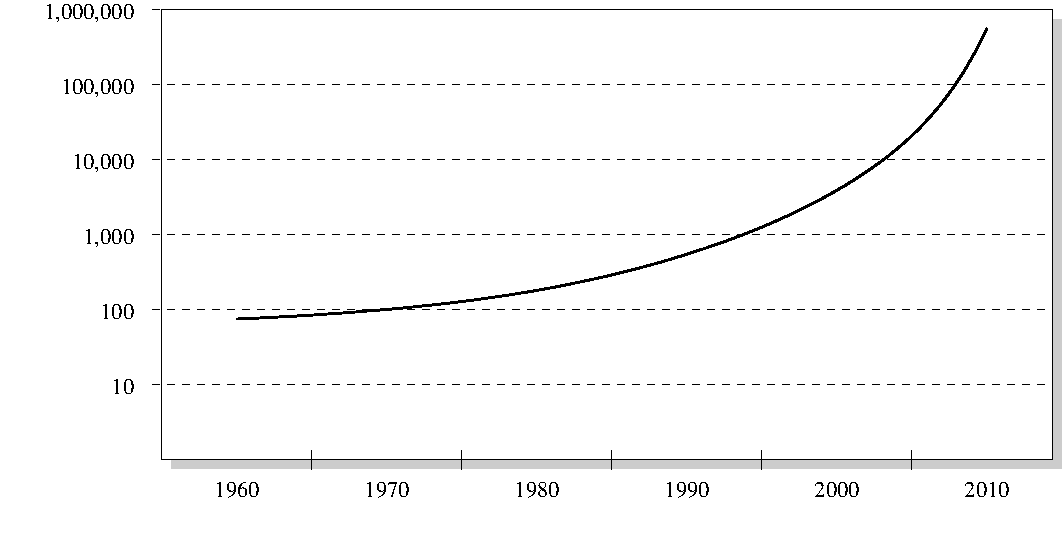
\includegraphics[width=\textwidth]{sa-sat-progress}\\
number of variables of a typical, practical SAT instance\\
that can be solved by the best solvers in that decade
\end{center}

\end{frame}

% ------------------------------------------------------------------------
% ------------------------------------------------------------------------
% ------------------------------------------------------------------------

\begin{frame}
\frametitle{Enabling Technology: SAT}

\begin{itemize}

\item propositional SAT solvers have made enourmous
progress in the last 10 years
\vfill

\item Further scalability improvements in recent years
because of efficient {\color{ta3skyblue}word-level reasoning} and
{\color{ta3skyblue}array decision procedures}

\end{itemize}

\end{frame}

% ------------------------------------------------------------------------
% ------------------------------------------------------------------------
% ------------------------------------------------------------------------

\begin{frame}
\frametitle{Let's Look at Another Path}

\begin{columns}
\begin{column}{.3\textwidth}
\only<1| handout:0>{\includegraphics{sha-example-0}}%
\only<2->{\includegraphics{sha-example-2}}
\end{column}
\begin{column}{.1\textwidth}
\pause\pause

\includegraphics[width=\textwidth]{arrow}
\end{column}
\begin{column}{.6\textwidth}
$\begin{array}{ll}
      & 0 \le t \le 79 \\
\land & t/20\not=0 \\
\land & t/20\not=1 \\
\land & t/20\not=2 \\
\land & t/20\not=3
\end{array}$\\[2ex]
\pause
That is UNSAT, so the assertion is unreachable.
\end{column}
\end{columns}

\end{frame}

% ------------------------------------------------------------------------
% ------------------------------------------------------------------------
% ------------------------------------------------------------------------

\begin{frame}[fragile]
\frametitle{What If a Variable is Assigned Twice?}

\begin{columns}
\begin{column}{.3\textwidth}
\begin{lstlisting}[language=C,basicstyle=\rmfamily,escapechar=\$,columns=flexible]
  x=0;

  if(y>=0)
    x++;
\end{lstlisting}
\end{column}
\begin{column}{.1\textwidth}

\includegraphics[width=\textwidth]{arrow}
\end{column}
\begin{column}{.5\textwidth}
Rename appropriately:
\[\begin{array}{ll}
      & x\only<2>{\alert{_1}}=0 \\
\land & y\only<2>{\alert{_0}}\ge 0 \\
\land & x\only<2>{\alert{_1}}=x\only<2>{\alert{_0}}+1
\end{array}\]
\end{column}
\end{columns}
\pause
\vfill
\begin{center}
This is a special case of \emph{SSA}
(static single assignment)
\end{center}

\end{frame}

% ------------------------------------------------------------------------
% ------------------------------------------------------------------------
% ------------------------------------------------------------------------

\begin{frame}[fragile]
\frametitle{Pointers}

How do we handle dereferencing in the program?
\pause\vfill

\begin{columns}
\begin{column}{.4\textwidth}
\begin{lstlisting}[language=C,basicstyle=\rmfamily,escapechar=\$,columns=flexible]
  int *p;
  p=malloc(sizeof(int)*5);
  ...

  p[1]=100;
\end{lstlisting}
\end{column}
\begin{column}{.1\textwidth}

\includegraphics[width=\textwidth]{arrow}
\end{column}
\begin{column}{.5\textwidth}
$\begin{array}{ll}
      & p_1=\&\mathit{DO1} \\
\land & \mathit{DO1}_1 = (\lambda i. \\
      &i=1?100: \mathit{DO1}_0[i])
\end{array}$
\end{column}
\end{columns}
\vfill

Track a `may-point-to' abstract state while simulating!

\end{frame}

% ------------------------------------------------------------------------
% ------------------------------------------------------------------------
% ------------------------------------------------------------------------

\begin{frame}
\frametitle{Scalability of Path Search}

Let's consider the following CFG:

\begin{center}
 \includegraphics{unrolling-cfg-0}
\end{center}

This is a loop with an {\tt if} inside.
\vfill
\pause

{\color{ta3scarletred}Q: how many paths for $n$ iterations?}

\end{frame}

% ------------------------------------------------------------------------
% ------------------------------------------------------------------------
% ------------------------------------------------------------------------

\section{BMC Basics}

\begin{frame}
\frametitle{Bounded Model Checking}

\begin{itemize}
\item Bounded Model Checking (BMC) is the most successful formal
validation technique in the \emph{hardware} industry
\vfill

\item Advantages:
\begin{itemize}
\item[\mycheck] \alert{Fully automatic}
\item[\mycheck] \alert{Robust}
\item[\mycheck] \alert{Lots of subtle bugs found}
\end{itemize}
\vfill

\item Idea: only look for bugs \alert{up to specific depth}
\vfill

\item Good for many applications, e.g., embedded systems

\end{itemize}
\end{frame}

% ------------------------------------------------------------------------
% ------------------------------------------------------------------------
% ------------------------------------------------------------------------

\begin{frame}
\frametitle{Transition Systems}

Definition: A transition system is a triple $(S, S_0, T)$ with
%
\begin{itemize}
\item set of states $S$,
\item a set of initial states $S_0\subset S$, and
\item a transition relation $T \subset (S\times S)$.
\end{itemize}
\vfill

The set $S_0$ and the relation $T$ can be written as
their characteristic functions.

\end{frame}

% ------------------------------------------------------------------------
% ------------------------------------------------------------------------
% ------------------------------------------------------------------------

\subsection{Unwinding a Transition System}

\begin{frame}
\frametitle{Unwinding a Transition System}

Q: How do we avoid the exponential path explosion?
\vfill

We just "{\color{ta3chameleon}concatenate}" the transition relation $T$:

\begin{center}
\begin{picture}(170,30)

\put(5,10){\circle*{5}}
\put(5,15){\makebox[0cm][c]{\small $S_0$}}

\pause
\put(10,10){\vector(1,0){30}}
\put(15,15){\makebox[0cm][c]{\small $\wedge$}}
\put(25,15){\makebox[0cm][c]{\small $T$}}
\put(45,10){\circle*{5}}

\pause
\put(45,15){\makebox[0cm][c]{\small $\wedge$}}
\put(65,15){\makebox[0cm][c]{\small $T$}}
\put(50,10){\vector(1,0){30}}
\put(85,10){\circle*{5}}

\pause
\put(105,10){\makebox[0cm][c]{\small $\ldots$}}
\put(85,15){\makebox[0cm][c]{\small $\wedge$}}

\put(125,10){\circle*{5}}
\put(130,10){\vector(1,0){30}}
\put(145,15){\makebox[0cm][c]{\small $T$}}
\put(125,15){\makebox[0cm][c]{\small $\wedge$}}

\put(165,10){\circle*{5}}

\pause
\put(5,0){\makebox[0cm][c]{\small $s_0$}}
\put(45,0){\makebox[0cm][c]{\small $s_1$}}
\put(85,0){\makebox[0cm][c]{\small $s_2$}}
\put(125,0){\makebox[0cm][c]{\small $s_{k-1}$}}
\put(165,0){\makebox[0cm][c]{\small $s_k$}}

\end{picture}
\end{center}

\end{frame}

% ------------------------------------------------------------------------
% ------------------------------------------------------------------------
% ------------------------------------------------------------------------

\begin{frame}
\frametitle{Unwinding a Transition System}

As formula:
\[ S_0(s_0) \land \bigwedge_{i=0}^{k-1} T(s_i,s_{i+1}) \]

\vfill
Satisfying assignments for this formula are \alert{traces}
through the transition system

\end{frame}

% ------------------------------------------------------------------------
% ------------------------------------------------------------------------
% ------------------------------------------------------------------------

\begin{frame}
\frametitle{Example}

\[ T \subseteq \mathds{N}_0 \times \mathds{N}_0 \]
\[ T(s,s') \iff s'.x=s.x+1 \]

\ldots and let $S_0(s)\iff s.x=0 \vee s.x=1$
\vfill
\pause

An unwinding for depth 4:
%
\[\begin{array}{ll}
      & (s_0.x=0  \vee s_0.x=1)\\
\land & s_1.x=s_0.x+1 \\
\land & s_2.x=s_1.x+1 \\
\land & s_3.x=s_2.x+1 \\
\land & s_4.x=s_3.x+1
\end{array}\]

\end{frame}

% ------------------------------------------------------------------------
% ------------------------------------------------------------------------
% ------------------------------------------------------------------------

\begin{frame}
\frametitle{Checking Reachability Properties}

Suppose we want to check a property of the form $\A\G p$.
\vfill
\pause

We then want at \alert{least one state} $s_i$ to satisfy $\neg p$:

\[ S_0(s_0) \land \bigwedge_{i=0}^{k-1} T(s_i,s_{i+1}) \quad\land\quad
\bigvee_{i=0}^k \neg p(s_i)
\]
\vfill

Satisfying assignments are \alert{counterexamples}
for the $\A\G p$ property

\end{frame}

% ------------------------------------------------------------------------
% ------------------------------------------------------------------------
% ------------------------------------------------------------------------

\subsection{Unwinding Software}

\begin{frame}
\frametitle{Unwinding Software}

We can do exactly that for our transition relation for software.
\vfill

E.g., for a program with 5 locations, 6 unwindings:

\begin{center}
\includegraphics[scale=.8]{unrolling-3}
\end{center}

\end{frame}

% ------------------------------------------------------------------------
% ------------------------------------------------------------------------
% ------------------------------------------------------------------------

\begin{frame}
\frametitle{Unwinding Software}

Problem: obviously, most of the formula is never 'used',\\
as only few sequences of PCs correspond to a path.

\end{frame}

% ------------------------------------------------------------------------
% ------------------------------------------------------------------------
% ------------------------------------------------------------------------

\begin{frame}
\frametitle{Unwinding Software}

Example:

\begin{center}
\begin{tabular}{ccc}
 \raisebox{.1cm}{\includegraphics{unrolling-0}}
&\raisebox{2cm}{\onslide<2>{
\includegraphics[scale=.5]{arrow}}}
&\onslide<2>{\includegraphics[scale=.8]{unrolling-4}} \\
CFG & & \onslide<2>{unrolling}
\end{tabular}
\end{center}

\end{frame}

% ------------------------------------------------------------------------
% ------------------------------------------------------------------------
% ------------------------------------------------------------------------

\begin{frame}
\frametitle{Unwinding Software}

Optimization:\\
{\color{ta3skyblue}don't generate the parts of the formula
that are not 'reachable'}

\begin{center}
\begin{tabular}{ccc}
 \raisebox{.1cm}{\includegraphics{unrolling-0}}
&\raisebox{2cm}{\onslide<2>{
\includegraphics[scale=.5]{arrow}}}
&\onslide<2>{\includegraphics[scale=.8]{unrolling-1}} \\
CFG & & \onslide<2>{unrolling}
\end{tabular}
\end{center}

\end{frame}

% ------------------------------------------------------------------------
% ------------------------------------------------------------------------
% ------------------------------------------------------------------------

\begin{frame}
\frametitle{Unwinding Software}

Problem:

\begin{center}
\begin{tabular}{ccc}
\includegraphics{unrolling-full-0}
&\raisebox{2cm}{
\includegraphics[scale=.5]{arrow}}
&\includegraphics[scale=.8]{unrolling-full-1} \\
CFG & & unrolling
\end{tabular}
\end{center}

\end{frame}

% ------------------------------------------------------------------------
% ------------------------------------------------------------------------
% ------------------------------------------------------------------------

\begin{frame}
\frametitle{Unwinding Software}

\begin{itemize}

\item Unwinding $T$ with bound $k$
results in a formula of size
\[ |T| \cdot k \]
\vfill

\item If we assume a $k$ that is only linear in $|T|$,\\
we get get a formula with size $O(|T|^2)$
\vfill

\item Can we do better?

\end{itemize}

\end{frame}

% ------------------------------------------------------------------------
% ------------------------------------------------------------------------
% ------------------------------------------------------------------------

\begin{frame}
\frametitle{Unrolling Loops}

Idea: do {\color{ta3chameleon}exactly one location} in each timeframe:

\begin{center}
\begin{tabular}{ccc}
 \raisebox{.1cm}{\includegraphics{unrolling-0}}
&\raisebox{2cm}{\onslide<2>{
\includegraphics[scale=.5]{arrow}}}
&\onslide<2>{\includegraphics[scale=.8]{unrolling-2}} \\
CFG & & \onslide<2>{unrolling}
\end{tabular}
\end{center}

\end{frame}

% ------------------------------------------------------------------------
% ------------------------------------------------------------------------
% ------------------------------------------------------------------------

\begin{frame}
\frametitle{Unrolling Loops}

\begin{itemize}

\item[\mycheck] More effective use of the formula size
\vfill

\item[\mycheck] Graph has fewer merge nodes,\\
the formula is easier for the solvers
\vfill

\item[\myfail] Not all paths of length $k$ are encoded\\
$\rightarrow$ the bound needs to be larger

\end{itemize}

\end{frame}

% ------------------------------------------------------------------------
% ------------------------------------------------------------------------
% ------------------------------------------------------------------------

\lstset{language=C,basicstyle=\rmfamily,escapechar=\$,columns=flexible}

\begin{frame}
\frametitle{Unrolling Loops}

This essentially amounts to unwinding loops:

\begin{center}
\colorbox{tabutter!50!white}{
\begin{picture}(200,170)
\put(0,0){\makebox(200,160)[tl]{\begin{minipage}[t]{\textwidth}
\only<1| handout:0>{%
\hspace*{0cm}  \lstinline!while(!\alert{cond}\lstinline!)!\\
\hspace*{.5cm} {\color{ta3chameleon}Body}\lstinline!;!
}%
\only<2| handout:0>{%
\hspace*{0cm}  \lstinline!if(!\alert{cond}\lstinline!) \{!\\
\hspace*{.5cm} {\color{ta3chameleon}Body}\lstinline!;!\\
\hspace*{.5cm} \lstinline!while(!\alert{cond}\lstinline!)!\\
\hspace*{1cm}  {\color{ta3chameleon}Body}\lstinline!;!\\
\hspace*{0cm}  \lstinline!\}!
}%
\only<3| handout:0>{%
\hspace*{0cm}  \lstinline!if(!\alert{cond}\lstinline!) \{!\\
\hspace*{.5cm} {\color{ta3chameleon}Body}\lstinline!;!\\
\hspace*{.5cm} \lstinline!if(!\alert{cond}\lstinline!) \{!\\
\hspace*{1cm}  {\color{ta3chameleon}Body}\lstinline!;!\\
\hspace*{1cm}  \lstinline!while(!\alert{cond}\lstinline!)!\\
\hspace*{1.5cm}{\color{ta3chameleon}Body}\lstinline!;!\\
\hspace*{.5cm} \lstinline!\}!\\
\hspace*{0cm}  \lstinline!\}!
}%
\only<4| handout:1>{%
\hspace*{0cm}  \lstinline!if(!\alert{cond}\lstinline!) \{!\\
\hspace*{.5cm} {\color{ta3chameleon}Body}\lstinline!;!\\
\hspace*{.5cm} \lstinline!if(!\alert{cond}\lstinline!) \{!\\
\hspace*{1cm}  {\color{ta3chameleon}Body}\lstinline!;!\\
\hspace*{1cm}  \lstinline!if(!\alert{cond}\lstinline!) \{!\\
\hspace*{1.5cm}{\color{ta3chameleon}Body}\lstinline!;!\\
\hspace*{1.5cm}\lstinline!while(!\alert{cond}\lstinline!)!\\
\hspace*{2cm}  {\color{ta3chameleon}Body}\lstinline!;!\\
\hspace*{1cm}  \lstinline!\}!\\
\hspace*{.5cm} \lstinline!\}!\\
\hspace*{0cm}  \lstinline!\}!
}%
\only<5| handout:0>{%
\hspace*{0cm}  \lstinline!if(!\alert{cond}\lstinline!) \{!\\
\hspace*{.5cm} {\color{ta3chameleon}Body}\lstinline!;!\\
\hspace*{.5cm} \lstinline!if(!\alert{cond}\lstinline!) \{!\\
\hspace*{1cm}  {\color{ta3chameleon}Body}\lstinline!;!\\
\hspace*{1cm}  \lstinline!if(!\alert{cond}\lstinline!) \{!\\
\hspace*{1.5cm}{\color{ta3chameleon}Body}\lstinline!;!\\
\hspace*{1.5cm}\lstinline!assume(!\alert{!cond}\lstinline!);!\\
\hspace*{2cm}  \\
\hspace*{1cm}  \lstinline!\}!\\
\hspace*{.5cm} \lstinline!\}!\\
\hspace*{0cm}  \lstinline!\}!
}%
\end{minipage}}}
\end{picture}}
\end{center}

\end{frame}

% ------------------------------------------------------------------------
% ------------------------------------------------------------------------
% ------------------------------------------------------------------------

\section{Completeness}

\begin{frame}
\frametitle{Completeness}

BMC, as discussed so far, is incomplete.\\
It only refutes, and does not
prove.
\vfill

How can we fix this?

\end{frame}

% ------------------------------------------------------------------------
% ------------------------------------------------------------------------
% ------------------------------------------------------------------------

\begin{comment}
\begin{frame}
\frametitle{Completeness: Overview}

We will see two techniques for making BMC for software
complete:
\vfill

\begin{enumerate}

\item Unwinding assertions
\vfill

\item $k$-induction

\end{enumerate}

\end{frame}
\end{comment}

% ------------------------------------------------------------------------
% ------------------------------------------------------------------------
% ------------------------------------------------------------------------

\subsection{Unwinding Assertions}

\begin{frame}
\frametitle{Unwinding Assertions}

Let's revisit the loop unwinding idea:

\begin{center}
\colorbox{tabutter!50!white}{
\begin{picture}(200,170)
\put(0,0){\makebox(200,160)[tl]{\begin{minipage}[t]{\textwidth}
\only<1| handout:0>{%
\hspace*{0cm}  \lstinline!while(!\alert{cond}\lstinline!)!\\
\hspace*{.5cm} {\color{ta3chameleon}Body}\lstinline!;!
}%
\only<2| handout:0>{%
\hspace*{0cm}  \lstinline!if(!\alert{cond}\lstinline!) \{!\\
\hspace*{.5cm} {\color{ta3chameleon}Body}\lstinline!;!\\
\hspace*{.5cm} \lstinline!while(!\alert{cond}\lstinline!)!\\
\hspace*{1cm}  {\color{ta3chameleon}Body}\lstinline!;!\\
\hspace*{0cm}  \lstinline!\}!
}%
\only<3| handout:0>{%
\hspace*{0cm}  \lstinline!if(!\alert{cond}\lstinline!) \{!\\
\hspace*{.5cm} {\color{ta3chameleon}Body}\lstinline!;!\\
\hspace*{.5cm} \lstinline!if(!\alert{cond}\lstinline!) \{!\\
\hspace*{1cm}  {\color{ta3chameleon}Body}\lstinline!;!\\
\hspace*{1cm}  \lstinline!while(!\alert{cond}\lstinline!)!\\
\hspace*{1.5cm}{\color{ta3chameleon}Body}\lstinline!;!\\
\hspace*{.5cm} \lstinline!\}!\\
\hspace*{0cm}  \lstinline!\}!
}%
\only<4| handout:1>{%
\hspace*{0cm}  \lstinline!if(!\alert{cond}\lstinline!) \{!\\
\hspace*{.5cm} {\color{ta3chameleon}Body}\lstinline!;!\\
\hspace*{.5cm} \lstinline!if(!\alert{cond}\lstinline!) \{!\\
\hspace*{1cm}  {\color{ta3chameleon}Body}\lstinline!;!\\
\hspace*{1cm}  \lstinline!if(!\alert{cond}\lstinline!) \{!\\
\hspace*{1.5cm}{\color{ta3chameleon}Body}\lstinline!;!\\
\hspace*{1.5cm}\lstinline!while(!\alert{cond}\lstinline!)!\\
\hspace*{2cm}  {\color{ta3chameleon}Body}\lstinline!;!\\
\hspace*{1cm}  \lstinline!\}!\\
\hspace*{.5cm} \lstinline!\}!\\
\hspace*{0cm}  \lstinline!\}!
}%
\only<5| handout:0>{%
\hspace*{0cm}  \lstinline!if(!\alert{cond}\lstinline!) \{!\\
\hspace*{.5cm} {\color{ta3chameleon}Body}\lstinline!;!\\
\hspace*{.5cm} \lstinline!if(!\alert{cond}\lstinline!) \{!\\
\hspace*{1cm}  {\color{ta3chameleon}Body}\lstinline!;!\\
\hspace*{1cm}  \lstinline!if(!\alert{cond}\lstinline!) \{!\\
\hspace*{1.5cm}{\color{ta3chameleon}Body}\lstinline!;!\\
\hspace*{1.5cm}\lstinline!assert(!\alert{!cond}\lstinline!);!\\
\hspace*{2cm}  \\
\hspace*{1cm}  \lstinline!\}!\\
\hspace*{.5cm} \lstinline!\}!\\
\hspace*{0cm}  \lstinline!\}!
}%
\end{minipage}}}
\end{picture}}
\end{center}

\end{frame}

% ------------------------------------------------------------------------
% ------------------------------------------------------------------------
% ------------------------------------------------------------------------

\begin{frame}
\frametitle{Unwinding Assertions}

\begin{itemize}
\item We replace the assumption we have used earlier to
cut off paths by an assertion
\vfill

\item[\mycheck] This allows us to
\alert{prove that we have done enough unwinding}
\vfill

\item This is a proof of a high-level worst-case execution time (WCET)
\vfill

\item Very appropriate for embedded software
\end{itemize}

\end{frame}

% ------------------------------------------------------------------------
% ------------------------------------------------------------------------
% ------------------------------------------------------------------------

\begin{comment}
\subsection{k-induction}

\begin{frame}
\frametitle{$k$-induction}


\end{frame}
\end{comment}

% ------------------------------------------------------------------------
% ------------------------------------------------------------------------
% ------------------------------------------------------------------------

\begin{frame}
\frametitle{CBMC Toolflow: Summary}

\begin{enumerate}

\item Parse, build CFG
\vfill

\item Unwind CFG, form formula
\vfill

\item Formula is solved by SAT/SMT

\end{enumerate}

\vfill

\begin{center}
\scalebox{.5}{\input{cbmc-flow.xfigtex}}
\end{center}

\end{frame}

% ------------------------------------------------------------------------
% ------------------------------------------------------------------------
% ------------------------------------------------------------------------

\section{Solving the Decision Problem}

\begin{frame}
\frametitle{Solving the Decision Problem}

Suppose we have used some unwinding, and have built the formula.
\vfill

For bit-vector arithmetic, the standard way of deciding satisfiability of
the formula is \emph{flattening},\\
followed by a call to a propositional SAT solver.
\vfill

In the SMT context: SMT-$\mathcal{BV}$

\end{frame}

% ------------------------------------------------------------------------
% ------------------------------------------------------------------------
% ------------------------------------------------------------------------

\begin{frame}

\frametitle{Bit-vector Flattening}

\begin{itemize}

\item This is easy for the bit-wise operators.
\vfill

\item 
Denote the Boolean variable for bit $i$ of term $t$ by \alert{$\mu(t)_i$}.
\vfill

\item Example for $a \,|_{[l]}\, b$:
%
\[ \bigwedge_{i=0}^{l-1} (\mu(t)_i=(a_i\vee b_i)) \]

(read $x=y$ over bits as $x \iff y$)

\pause
\vfill

\item We can transform this into CNF using Tseitin's method.

\end{itemize}

\end{frame}

% ------------------------------------------------------------------------
% ------------------------------------------------------------------------
% ------------------------------------------------------------------------

\begin{frame}

\frametitle{Flattening Bit-Vector Arithmetic}

How to flatten \alert{$a+b$}?

\pause

\vspace*{1ex}

$\longrightarrow$ we can build a \emph{circuit} that adds them!
\vfill

\begin{columns}

\begin{column}{1.5cm}

\scalebox{0.75}{
\setlength{\unitlength}{0.00083333in}
%
{\renewcommand{\dashlinestretch}{30}
\begin{picture}(624,1710)(0,-10)
\path(162,525)(162,225)
\put(140,700){\makebox(0,0)[lb]{{\SetFigFont{20}{24.0}{\sfdefault}{\mddefault}{\updefault}FA}}}
\put(499,1500){\makebox(0,0)[lb]{{\SetFigFont{17}{20.4}{\rmdefault}{\mddefault}{\itdefault}i}}}
\put(262,1500){\makebox(0,0)[lb]{{\SetFigFont{17}{20.4}{\rmdefault}{\mddefault}{\itdefault}b}}}
\put(28,1500){\makebox(0,0)[lb]{{\SetFigFont{17}{20.4}{\rmdefault}{\mddefault}{\itdefault}a}}}
\put(407,0){\makebox(0,0)[lb]{{\SetFigFont{17}{20.4}{\rmdefault}{\mddefault}{\itdefault}s}}}
\put(86,0){\makebox(0,0)[lb]{{\SetFigFont{17}{20.4}{\rmdefault}{\mddefault}{\itdefault}o}}}
\path(87,1425)(87,1125)
\path(312,1425)(312,1125)
\path(537,1425)(537,1125)
\path(462,525)(462,225)
\path(12,1125)(612,1125)(612,525)(12,525)(12,1125)
\end{picture}}}

\end{column}

\begin{column}{9cm}

\begin{block}{Full Adder}
$\begin{array}{r@{\quad}c@{\quad}l@{\quad}c@{\quad}l}
s &\equiv& (a + b + i \;) \mathrel{\mathrm{mod}} 2 &\equiv& a \oplus b \oplus i
\\[1.5ex]
\mathit{o} &\equiv& (a + b + i\;) \mathrel{\mathrm{div}} 2 &\equiv&
a \cdot b + a \cdot i + b \cdot i
\end{array}$
\end{block}

\end{column}
\end{columns}
\vfill

The full adder in CNF:
%
\[\begin{array}{l}
(     a \lor      b \lor             \neg o) \land
(     a \lor \neg b \lor      i \lor \neg o) \land
(     a \lor \neg b \lor \neg i \lor      o) \land\\
(\neg a \lor      b \lor      i \lor \neg o) \land
(\neg a \lor      b \lor \neg i \lor      o) \land
(\neg a \lor \neg b \lor                  o)
\end{array}\]

\end{frame}

% ------------------------------------------------------------------------
% ------------------------------------------------------------------------
% ------------------------------------------------------------------------

\begin{frame}

\frametitle{Flattening Bit-Vector Arithmetic}

Ok, this is good for one bit! How about more?

\pause

\vspace*{2ex}

\begin{block}{8-Bit ripple carry adder (RCA)}

\begin{center}
\scalebox{0.65}{
\setlength{\unitlength}{0.00083333in}
{\renewcommand{\dashlinestretch}{30}
\begin{picture}(7640,1785)(0,-10)
\path(3214,1425)(3214,1125)
\path(6289,525)(6289,225)
\path(5914,1425)(5914,1125)
\path(6139,1425)(6139,1125)
\path(5989,525)(5989,375)(5689,375)
	(5689,1275)(5464,1275)(5464,1125)
\path(5389,525)(5389,225)
\path(5014,1425)(5014,1125)
\path(5239,1425)(5239,1125)
\path(7189,525)(7189,225)
\path(6814,1425)(6814,1125)
\path(7039,1425)(7039,1125)
\path(6889,525)(6889,375)(6589,375)
	(6589,1275)(6364,1275)(6364,1125)
\path(7189,1125)(7189,1275)(7489,1275)
\path(589,525)(589,375)(289,375)
\path(889,525)(889,225)
\path(739,1425)(739,1125)
\path(1489,525)(1489,375)(1189,375)
	(1189,1275)(964,1275)(964,1125)
\path(1789,525)(1789,225)
\path(1639,1425)(1639,1125)
\path(2389,525)(2389,375)(2089,375)
	(2089,1275)(1864,1275)(1864,1125)
\path(2689,525)(2689,225)
\path(2539,1425)(2539,1125)
\path(3289,525)(3289,375)(2989,375)
	(2989,1275)(2764,1275)(2764,1125)
\path(3589,525)(3589,225)
\path(3439,1425)(3439,1125)
\path(4189,525)(4189,375)(3889,375)
	(3889,1275)(3664,1275)(3664,1125)
\path(4489,525)(4489,225)
\path(4339,1425)(4339,1125)
\path(5089,525)(5089,375)(4789,375)
	(4789,1275)(4564,1275)(4564,1125)
\path(439,1125)(1039,1125)(1039,525)
	(439,525)(439,1125)
\path(1339,1125)(1939,1125)(1939,525)
	(1339,525)(1339,1125)
\path(1414,1425)(1414,1125)
\path(514,1425)(514,1125)
\path(2239,1125)(2839,1125)(2839,525)
	(2239,525)(2239,1125)
\path(3139,1125)(3739,1125)(3739,525)
	(3139,525)(3139,1125)
\path(4114,1425)(4114,1125)
\path(4939,1125)(5539,1125)(5539,525)
	(4939,525)(4939,1125)
\path(4039,1125)(4639,1125)(4639,525)
	(4039,525)(4039,1125)
\path(5839,1125)(6439,1125)(6439,525)
	(5839,525)(5839,1125)
\path(6739,1125)(7339,1125)(7339,525)
	(6739,525)(6739,1125)
\put(7564,1200){\makebox(0,0)[lb]{{\SetFigFont{17}{20.4}{\rmdefault}{\mddefault}{\itdefault}$i$}}}
\put(739,705){\makebox(0,0)[b]{{\SetFigFont{20}{24.0}{\sfdefault}{\mddefault}{\updefault}FA}}}
\put(1639,705){\makebox(0,0)[b]{{\SetFigFont{20}{24.0}{\sfdefault}{\mddefault}{\updefault}FA}}}
\put(2539,705){\makebox(0,0)[b]{{\SetFigFont{20}{24.0}{\sfdefault}{\mddefault}{\updefault}FA}}}
\put(3439,705){\makebox(0,0)[b]{{\SetFigFont{20}{24.0}{\sfdefault}{\mddefault}{\updefault}FA}}}
\put(4339,705){\makebox(0,0)[b]{{\SetFigFont{20}{24.0}{\sfdefault}{\mddefault}{\updefault}FA}}}
\put(5239,705){\makebox(0,0)[b]{{\SetFigFont{20}{24.0}{\sfdefault}{\mddefault}{\updefault}FA}}}
\put(6139,705){\makebox(0,0)[b]{{\SetFigFont{20}{24.0}{\sfdefault}{\mddefault}{\updefault}FA}}}
\put(7039,705){\makebox(0,0)[b]{{\SetFigFont{20}{24.0}{\sfdefault}{\mddefault}{\updefault}FA}}}
\put(514,1500){\makebox(0,0)[b]{{\SetFigFont{17}{20.4}{\rmdefault}{\mddefault}{\itdefault}$a_7$}}}
\put(739,1500){\makebox(0,0)[b]{{\SetFigFont{17}{20.4}{\rmdefault}{\mddefault}{\itdefault}$b_7$}}}
\put(1414,1500){\makebox(0,0)[b]{{\SetFigFont{17}{20.4}{\rmdefault}{\mddefault}{\itdefault}$a_6$}}}
\put(1639,1500){\makebox(0,0)[b]{{\SetFigFont{17}{20.4}{\rmdefault}{\mddefault}{\itdefault}$b_6$}}}
\put(2314,1500){\makebox(0,0)[b]{{\SetFigFont{17}{20.4}{\rmdefault}{\mddefault}{\itdefault}$a_5$}}}
\put(2539,1500){\makebox(0,0)[b]{{\SetFigFont{17}{20.4}{\rmdefault}{\mddefault}{\itdefault}$b_5$}}}
\put(3214,1500){\makebox(0,0)[b]{{\SetFigFont{17}{20.4}{\rmdefault}{\mddefault}{\itdefault}$a_4$}}}
\put(3439,1500){\makebox(0,0)[b]{{\SetFigFont{17}{20.4}{\rmdefault}{\mddefault}{\itdefault}$b_4$}}}
\put(4114,1500){\makebox(0,0)[b]{{\SetFigFont{17}{20.4}{\rmdefault}{\mddefault}{\itdefault}$a_3$}}}
\put(4339,1500){\makebox(0,0)[b]{{\SetFigFont{17}{20.4}{\rmdefault}{\mddefault}{\itdefault}$b_3$}}}
\put(5014,1500){\makebox(0,0)[b]{{\SetFigFont{17}{20.4}{\rmdefault}{\mddefault}{\itdefault}$a_2$}}}
\put(5239,1500){\makebox(0,0)[b]{{\SetFigFont{17}{20.4}{\rmdefault}{\mddefault}{\itdefault}$b_2$}}}
\put(5914,1500){\makebox(0,0)[b]{{\SetFigFont{17}{20.4}{\rmdefault}{\mddefault}{\itdefault}$a_1$}}}
\put(6139,1500){\makebox(0,0)[b]{{\SetFigFont{17}{20.4}{\rmdefault}{\mddefault}{\itdefault}$b_1$}}}
\put(6814,1500){\makebox(0,0)[b]{{\SetFigFont{17}{20.4}{\rmdefault}{\mddefault}{\itdefault}$a_0$}}}
\put(7039,1500){\makebox(0,0)[b]{{\SetFigFont{17}{20.4}{\rmdefault}{\mddefault}{\itdefault}$b_0$}}}
\put(139,331){\makebox(0,0)[rb]{{\SetFigFont{17}{20.4}{\rmdefault}{\mddefault}{\itdefault}$o$}}}
\put(889,0){\makebox(0,0)[b]{{\SetFigFont{17}{20.4}{\rmdefault}{\mddefault}{\itdefault}$s_7$}}}
\put(1789,0){\makebox(0,0)[b]{{\SetFigFont{17}{20.4}{\rmdefault}{\mddefault}{\itdefault}$s_6$}}}
\put(2689,0){\makebox(0,0)[b]{{\SetFigFont{17}{20.4}{\rmdefault}{\mddefault}{\itdefault}$s_5$}}}
\put(3589,0){\makebox(0,0)[b]{{\SetFigFont{17}{20.4}{\rmdefault}{\mddefault}{\itdefault}$s_4$}}}
\put(4489,0){\makebox(0,0)[b]{{\SetFigFont{17}{20.4}{\rmdefault}{\mddefault}{\itdefault}$s_3$}}}
\put(5389,0){\makebox(0,0)[b]{{\SetFigFont{17}{20.4}{\rmdefault}{\mddefault}{\itdefault}$s_2$}}}
\put(6289,0){\makebox(0,0)[b]{{\SetFigFont{17}{20.4}{\rmdefault}{\mddefault}{\itdefault}$s_1$}}}
\put(7189,0){\makebox(0,0)[b]{{\SetFigFont{17}{20.4}{\rmdefault}{\mddefault}{\itdefault}$s_0$}}}
\path(2314,1425)(2314,1125)
\end{picture}}}
\end{center}

\end{block}

\begin{itemize}

\item Also called \emph{carry chain adder}

\item Adds $l$ variables

\item Adds $6\cdot l$ clauses

\end{itemize}

\end{frame}

% ------------------------------------------------------------------------
% ------------------------------------------------------------------------
% ------------------------------------------------------------------------

\subsection{Incremental Flattening}

\begin{frame}

\frametitle{Multipliers}

\begin{itemize}

\item \alert{Multipliers} result in very hard formulas
\vfill

\item Example:
%
\[ a\cdot b=c \,\land\, b\cdot a\not =c \,\land\, x<y \,\land\, x>y \]

CNF: About 11000 variables,\\
\alert{unsolvable} for current SAT solvers
\vfill

\item Similar problems with division, modulo
\vfill

\item Q: Why is this hard?

\pause

\item Q: How do we fix this?

\end{itemize}

\end{frame}

% ------------------------------------------------------------------------
% ------------------------------------------------------------------------
% ------------------------------------------------------------------------

\begin{frame}

\frametitle{Incremental Flattening}

\begin{center}
\begin{picture}(270,150)

\put(60,150){\vector(0,-1){10}}
\put(60,120){\makebox[0cm][c]{
\includegraphics[height=20pt,width=90pt]{gradient_box_yellow}}}
\put(60,127){\makebox[0cm][c]{$\varphi_f:=\varphi_\mathit{sk}$, $F:=\emptyset$}}

\onslide<2->{
\put(60,120){\vector(0,-1){60}}
\put(60,40){\makebox[0cm][c]{
\includegraphics[height=20pt,width=90pt]{gradient_box_red}}}
\put(60,47){\makebox[0cm][c]{Is $\varphi_f$ SAT?}}
}

\onslide<3->{
\put(60,40){\vector(0,-1){30}}
\put(62,20){No!}
\put(60,0){\makebox[0cm][c]{\color{tascarletred}UNSAT}}
}

\onslide<4->{
\put(105,50){\vector(1,0){45}}
\put(115,52){Yes!}
\put(150,40){
\includegraphics[height=20pt,width=80pt]{gradient_box_green}}
\put(190,47){\makebox[0cm][c]{compute $I$}}
}

\onslide<5->{
\put(190,40){\vector(0,-1){30}}
\put(192,20){$I=\emptyset$}
\put(190,0){\makebox[0cm][c]{\color{tascarletred}SAT}}
}

\onslide<6->{
\put(190,60){\vector(0,1){20}}
\put(192,65){$I\not=\emptyset$}
\put(120,80){
\includegraphics[height=40pt,width=140pt]{gradient_box_yellow}}
\put(190,108){\makebox[0cm][c]{Pick $F'\subseteq(I\setminus F)$}}
\put(190,96){\makebox[0cm][c]{$F:=F\cup F'$}}
\put(190,85){\makebox[0cm][c]{$\varphi_f:=\varphi_f \land \textsc{Constraint}(F)$}}
\put(120,100){\vector(-1,0){60}}
}

\end{picture}
\end{center}

\onslide<1->{$\varphi_\mathit{sk}$: Boolean part of $\varphi$\\
$F$: set of terms that are in the encoding\\}
\onslide<4->{$I$: set of terms that are inconsistent with the current assignment}

\end{frame}

% ------------------------------------------------------------------------
% ------------------------------------------------------------------------
% ------------------------------------------------------------------------

\begin{frame}

\frametitle{Incremental Flattening}

\begin{itemize}

\item Idea: add 'easy' parts of the formula first
\vfill

\item Only add hard parts when needed
\vfill

\item $\varphi_f$ only gets stronger -- use an \alert{incremental SAT
solver}

\end{itemize}

\end{frame}

% ------------------------------------------------------------------------
% ------------------------------------------------------------------------
% ------------------------------------------------------------------------

\end{document}
